\subsection{Prestazioni}
Il sistema è stato analizzato eseguendo client e server sulla stessa 
macchina, sfruttando l'interfaccia di loopback.\\
Le prestazioni sono state analizzate facendo variare i paramatri T, P e N
uno alla volta.\\
Per effettuare un'analisi automatica e soddisfacente delle prestazioni 
sono stati opportunamente modificati i moduli \emph{server.c} e 
\emph{client.c}.\\
Il server è stato modificato in modo che facesse variare il parametro
desiderato ad ogni richiesta di un client. In altre parole si ottiene
un insieme di processi che gestiscono ognuno una connessione con un valore
del parametro diverso.
\begin{lstlisting}[title=server\_test.c]
    .....

for (params.N = MIN_WIDTH; params.N <= MAX_WIDTH; params.N += 10) {
//for (params.T = MIN_TIMEOUT; params.T < MAX_TIMEOUT; 
//     params.T += 100) {
//for (params.P = MIN_LOSS; params.P < MAX_LOSS; params.P += 10) {

	/* wait for connection requests */

	/* create a new proccess to handle the client requests */
	pid = fork();

	.....

	if (!pid) {             // child process

		create_test_connection(&params, &cliaddr, clilen);
		server_job();
	}
}
.....
\end{lstlisting}
Lato client è stata implementata un'applicazione che genera processi 
client i quali si connettono sequenzialmente al server. Questi  
effettuano una richiesta GET dello stesso file ``test'' e al termine
scrivono il tempo impiegato su di un file.
Il file in questione ha dimensioni pari a 1.4 MiB, così ridotte 
affinché sia possibile eseguire i test anche per probabilità elevate di
perdita in tempi ragionevoli.
\begin{lstlisting}[title=client\_test.c]
int main()
{
    .....

    for (;;) {

        // create child 
        pid = fork();

        if (!pid) {
            // create a new socket  
            .....
            create_test_connection(sockfd, &servaddr);

			close(sockfd);
			exit(EXIT_SUCCESS);
        }
        // wait for child termination 
        if (wait(NULL) == -1)
            handle_error("wait");
    }
    exit(EXIT_SUCCESS);
}

void create_test_connection(int sockfd, struct sockaddr_in *addr)
{
    .....

    /* send SYN */
    .....
    /* get SYN_ACK and server connection address */
    .....
    /* set the endpoint */
    .....

    /* initialize transport layer */
    init_transport(sockfd, &params);
    test_job(&params);
}

void test_job(struct proto_params *params)
{
    struct timespec start, end, elapsed;
    char *filename = "test";
    FILE *file = fopen("test_files/test.dat", "a");
    if (!file)
        handle_error("fopen()");

    if (clock_gettime(CLOCK_REALTIME, &start) == -1)
        handle_error("getting test start time");

    cli_get(filename);

    if (clock_gettime(CLOCK_REALTIME, &end) == -1)
        handle_error("getting test end time");
    if (timespec_sub(&elapsed, &end, &start) == -1)
        handle_error("calculating test elapsed time");

    fprintf(file, "%u ", params->N);
    //fprintf(file, "%u ", params->P);
    //fprintf(file, "%u ", params->T);

    fprint_timespec(file, &elapsed);

    fclose(file);
}
\end{lstlisting}
%
\subsubsection{Analisi al variare di N}
L'analisi delle prestazioni al variare del parametro N sono state svolte in 
condizioni di vario tipo, ma in ogni caso si osserva chiaramente che il tempo
impiegato decresce esponenzialmente all'aumentare dell'ampiezza della finestra
N.\\
Confrontando i due tipo di algoritmi, con timeout addatativo e non, si osserva
che per un timeout iniziale di 500 millisecondi, quello di tipo adattativo 
ottiene performance migliori in ogni caso, mentre per un timeout iniziale di 
250 millisecondi, che è il valore di soglia minimo, l'adattativo converge 
alla versione con timeout fisso solo in condizioni di basse e medie probabilità di 
perdita. In condizioni di perdite frequenti (70\%) ottiene performance peggiori ed 
in alcuni casi il grafico è soggetto a picchi. La causa di questo comportamento 
potrebbe essere legata al fatto che, in casi di perdite frequenti, si verificano
altrettanto frequentemente invii e e ritrasmissioni di un gran numero di pacchetti.
Questi eventi trattengono il servizio di invio impegnato abbastanza a lungo,
essendo inoltre operazioni di scrittura su file (socket), da
ritardare il timestamp relativo all'arrivo di eventuali ack, con conseguente 
errore sul calcolo dell'RTT e quindi aumento del timeout.
\begin{figure}[!hp]
	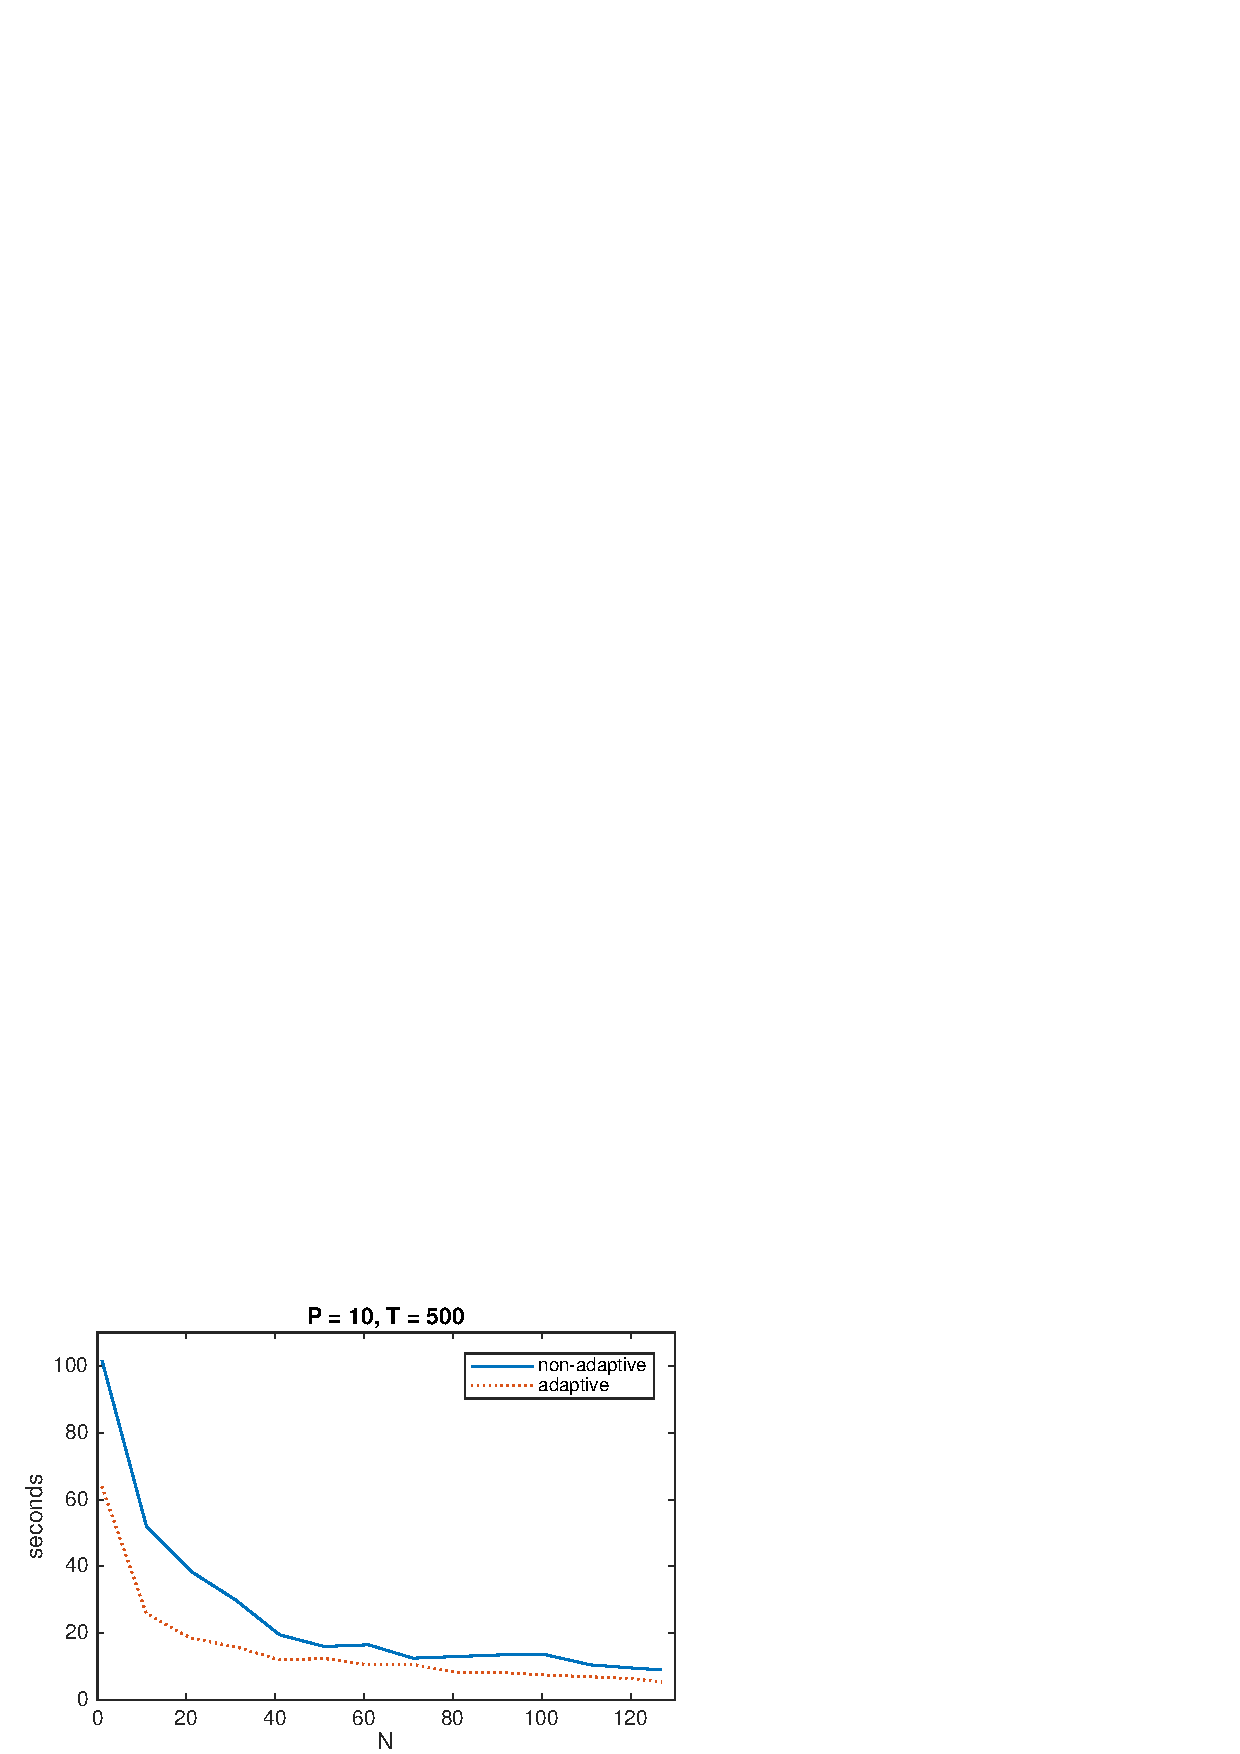
\includegraphics[scale=0.5]{images/N_T500_P10}
	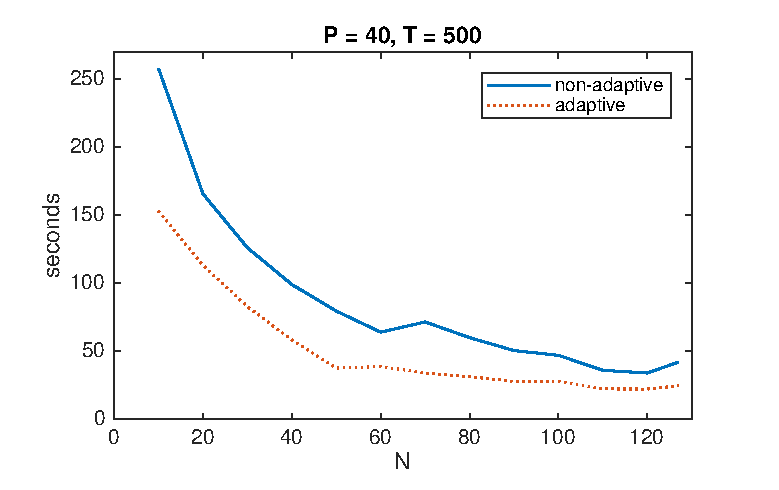
\includegraphics[scale=0.5]{images/N_T500_P40}
	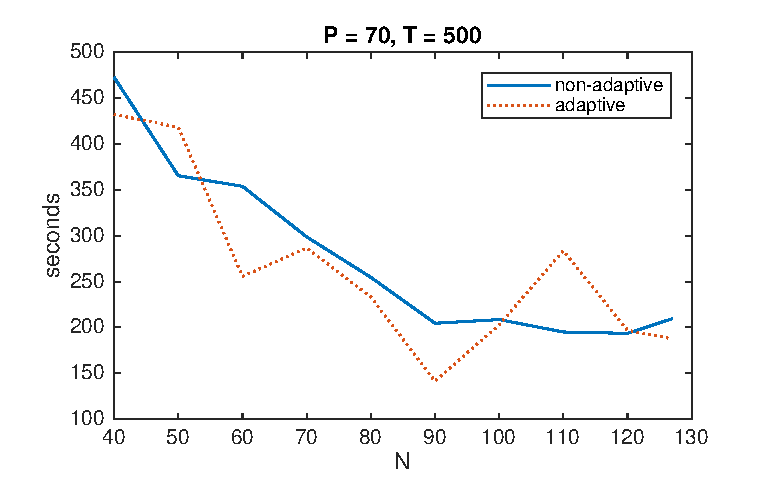
\includegraphics[scale=0.5]{images/N_T500_P70}
	\caption{prestazioni al variare dell'ampiezza della finestra N,
			 timeout T = 500 ms, probabilità di perdita bassa (P = 10\%),
			 media (P = 40\%) e alta (P = 70\%)}
\end{figure}
\begin{figure}[!hp]
	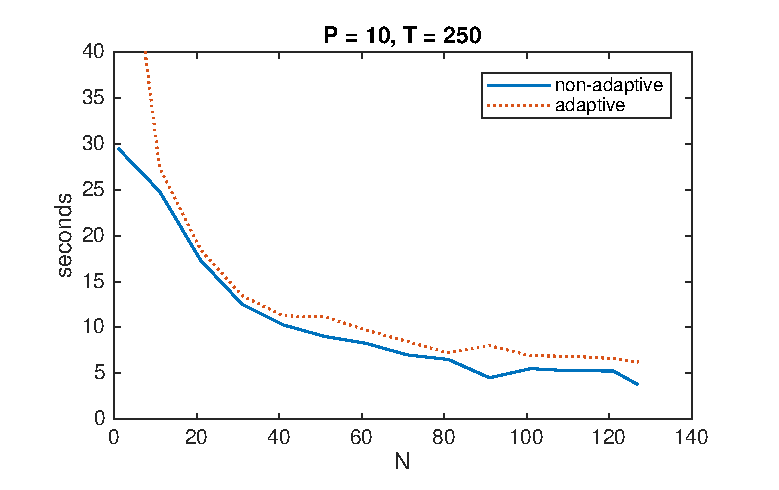
\includegraphics[scale=0.5]{images/N_T250_P10}
	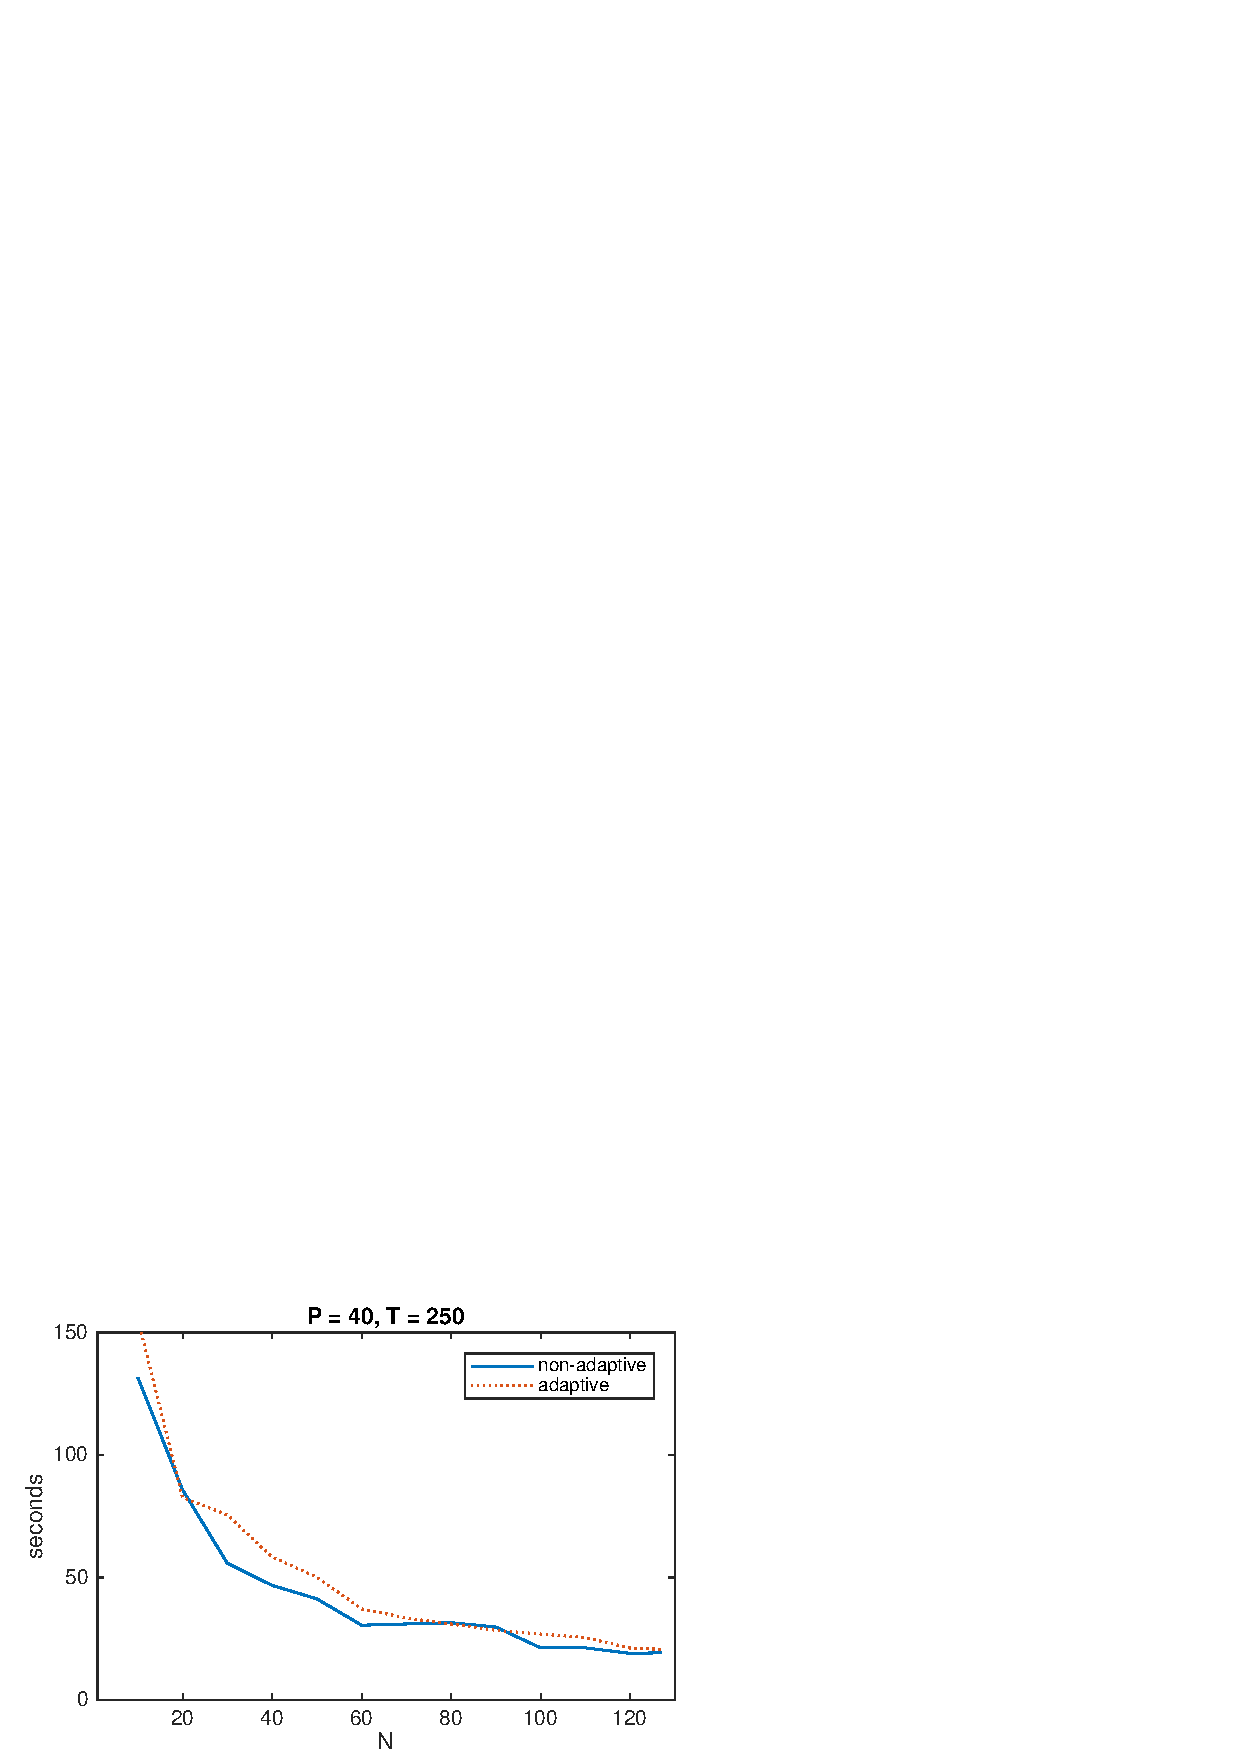
\includegraphics[scale=0.5]{images/N_T250_P40}
	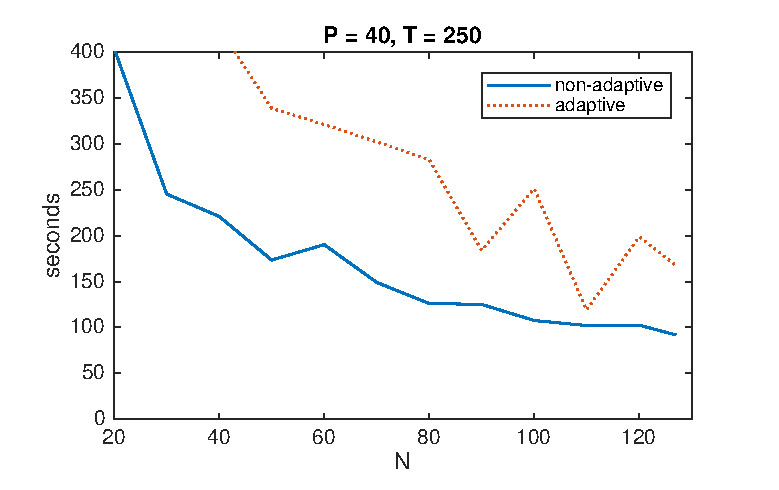
\includegraphics[scale=0.5]{images/N_T250_P70}
	\caption{prestazioni al variare dell'ampiezza della finestra N,
			 timeout T = 250 ms, probabilità di perdita bassa (P = 10\%),
			 media (P = 40\%) e alta (P = 70\%)}
\end{figure}

\subsubsection{Analisi al variare di T}
Per quanto riguarda le prestazioni al variare del valore del timeout,
si osserva (figura \ref{t}) che vi è una crescita lineare del tempo impiegato all'aumentare del
parametro T nel caso di timeout fisso.\\
Nel caso di timeout adattativo, per perdite poco o mediamente frequenti,
il tempo impiegato converge ad un valore costante
proporzionale alla probabilità di perdita,
mentre si conferma molto variabile in caso di elevata probabilità di perdita. 
\begin{figure}[!hp]
	\centering
	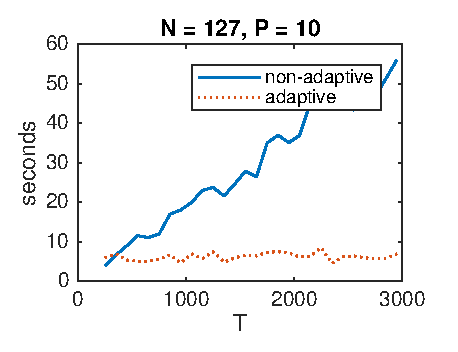
\includegraphics[scale=0.8]{images/T_N127_P10}
	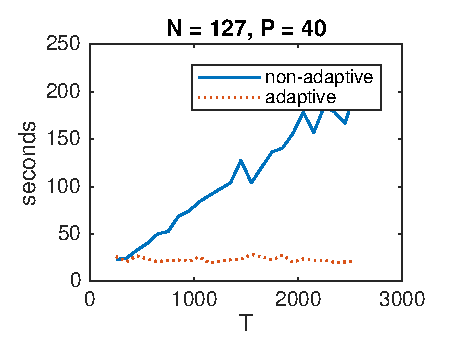
\includegraphics[scale=0.8]{images/T_N127_P40}
	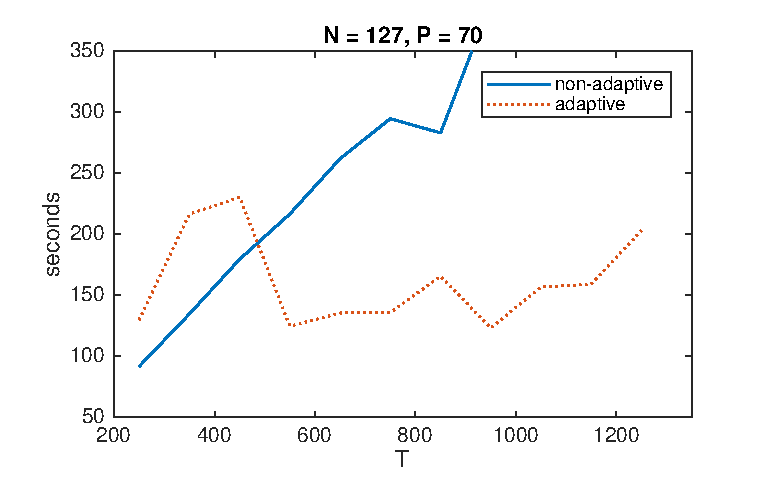
\includegraphics[scale=0.8]{images/T_N127_P70}
	\caption{prestazioni al variare del valore del timeout T,
			 ampiezza finestra N = 127, probabilità di perdita bassa (P = 10\%),
			 media (P = 40\%) e alta (P = 70\%)}
	\label{t}
\end{figure}

\subsubsection {Analisi al variare di P}
Anche al variare della probabilità di perdità si osserva un andamento 
abbastanza lineare fino a valori vicini al 60\%, da questo punto in
poi però, si ha una rapida divergenza e le prestazioni peggiorano
drasticamente.\\
Confermate, anche in questo caso, le peggiori prestazioni della versione
con timeout adattativo rispetto a timeout fisso per probabilità di perdita
elevate.
\begin{figure}[!ht]
	\centering
	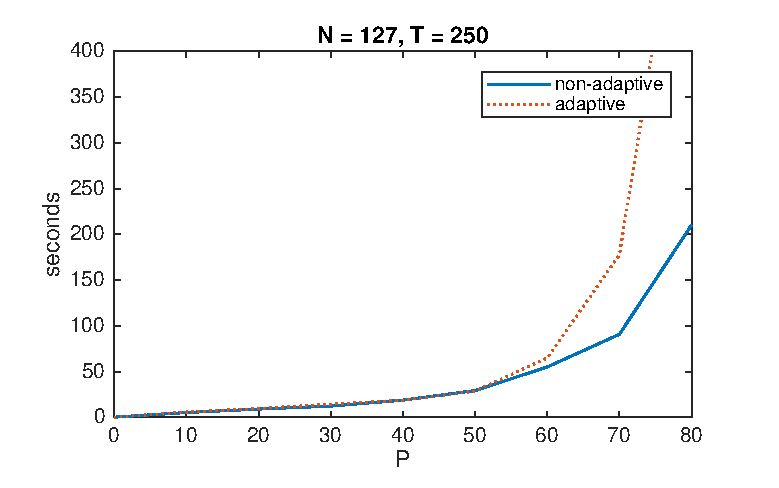
\includegraphics[scale=0.8]{images/P_N127_T250}
	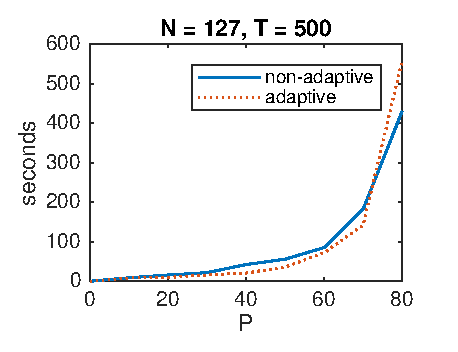
\includegraphics[scale=0.8]{images/P_N127_T500}
	\caption{prestazioni al variare della probabilità di perdita P,
			 ampiezza finestra N = 127, timeout minimo T = 250 ms e 
			 timeout normale T = 500 ms}
\end{figure}
\newpage

%
